%%%%%%%%%%%%%%%%%%%%%%%%%%%%%%%%%%%%%%%%%
% Structured General Purpose Assignment
% LaTeX Template
%
% This template has been downloaded from:
% http://www.latextemplates.com
%
% Original author:
% Ted Pavlic (http://www.tedpavlic.com)
%
% Note:
% The \lipsum[#] commands throughout this template generate dummy text
% to fill the template out. These commands should all be removed when 
% writing assignment content.
%
%%%%%%%%%%%%%%%%%%%%%%%%%%%%%%%%%%%%%%%%%

\documentclass{article}

\usepackage{fancyhdr} % Required for custom headers
\usepackage{lastpage} % Required to determine the last page for the footer
\usepackage{extramarks} % Required for headers and footers
\usepackage{graphicx} % Required to insert images
\usepackage[latin1]{inputenc}

% Margins
\topmargin=-0.45in
\evensidemargin=0in
\oddsidemargin=0in
\textwidth=6.5in
\textheight=9.0in
\headsep=0.25in 

\linespread{1.1} % Line spacing



\setlength\parindent{0pt} % Removes all indentation from paragraphs

%----------------------------------------------------------------------------------------
%	DOCUMENT STRUCTURE COMMANDS
%	Skip this unless you know what you're doing
%----------------------------------------------------------------------------------------

% Header and footer for when a page split occurs within a problem environment
\newcommand{\enterProblemHeader}[1]{
\nobreak\extramarks{#1}{#1 continued on next page\ldots}\nobreak
\nobreak\extramarks{#1 (continued)}{#1 continued on next page\ldots}\nobreak
}

% Header and footer for when a page split occurs between problem environments
\newcommand{\exitProblemHeader}[1]{
\nobreak\extramarks{#1 (continued)}{#1 continued on next page\ldots}\nobreak
\nobreak\extramarks{#1}{}\nobreak
}

\setcounter{secnumdepth}{0} % Removes default section numbers
\newcounter{homeworkProblemCounter} % Creates a counter to keep track of the number of problems
%----------------------------------------------------------------------------------------
%	NAME AND CLASS SECTION
%----------------------------------------------------------------------------------------

\newcommand{\lessonNumber}[1]{Lezione\ \##1} % Assignment title
\newcommand{\lessonDate}[4]{#1,\ #2\ #3\ #4} % Due date
\newcommand{\lessonCourse}[1]{#1} % Course/class
\newcommand{\lessonTime}[1]{#1} % Class/lecture time
\newcommand{\lessonTeacher}[1]{#1} % Teacher/lecturer
\newcommand{\lessonAuthor}[1]{#1} % Your name

% Set up the header and footer
\pagestyle{fancy}
\lhead{\lessonAuthor{Luca De Franceschi}} % Top left header
\chead{\lessonAuthor{Christian Cardin}\ \lessonTime{9:30}: \lessonNumber{17}} % Top center header
\rhead{\firstxmark} % Top right header
\lfoot{\lastxmark} % Bottom left footer
\cfoot{} % Bottom center footer
\rfoot{Page\ \thepage\ of\ \pageref{LastPage}} % Bottom right footer
\renewcommand\headrulewidth{0.4pt} % Size of the header rule
\renewcommand\footrulewidth{0.4pt} % Size of the footer rule

%----------------------------------------------------------------------------------------
%	TITLE PAGE
%----------------------------------------------------------------------------------------

\title{
\vspace{2in}
\textmd{\textbf{\lessonNumber{17}}\\
\normalsize\vspace{0.1in}\small{\lessonDate{Lunedì}{18}{Novembre}{2013}}\\
\vspace{0.1in}\large{\textit{\lessonTeacher{Christian Cardin},\ \lessonTime{09:30-11:15}}}
\vspace{3in}
}
}

\author{\textbf{\lessonAuthor{Luca De Franceschi}}}
\date{} % Insert date here if you want it to appear below your name

%----------------------------------------------------------------------------------------

\begin{document}

\maketitle
\newpage
\newpage

\textbf{Esercizio} (biglietti aerei):

\begin{center}

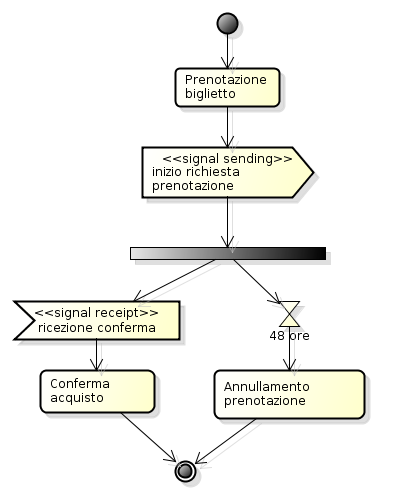
\includegraphics[width=0.75\columnwidth]{img1} % Example image

\end{center}

\textbf{Diagrammi dei package}\\\\

Non li troveremo mai dai soli perchè storicamente i package viaggiano con le classi, ma da UML2 possono contenere qualsiasi cosa; sono usati spesso nella parte architetturale, ci permettono di tenere sotto controllo la complessità del sistema che si misura con le dipendenze. Un package non è altro che un raggruppamento di elementi UML. In effetti andremo a raggruppare solo classi. I rapporti tra package UML e package di linguaggio di programmazione è molto stretto, quasi 1:1. Il package si presenta come una grande cartella che ha un titolo e contiene al suo interno classi o altri package. Una classe appartiene ad un solo package. Il package individua un \textit{namespace}, ogni elemento deve avere un nome distinto all'interno dello spazio dei nomi. In UML per riferirsi ad un nome qualificato si usa la notazione dei ::.

\begin{center}

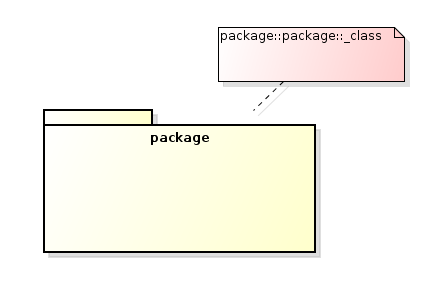
\includegraphics[width=0.75\columnwidth]{img2} % Example image

\end{center}

L'interfaccia di un package è l'insieme delle classi che hanno visibilità pubblica di un package.\\
Principi di progettazione:

\begin{itemize}

	\item \textbf{Common Closure Principle}, classi dello stesso package condividono la stessa causa di cambiamento;
	\item \textbf{Common Reuse Principle}, classi dello stesso package dovrebbero sempre essere riusate insieme.

\end{itemize}

I package possono avere \textbf{dipendenze} tra loro:

\begin{center}

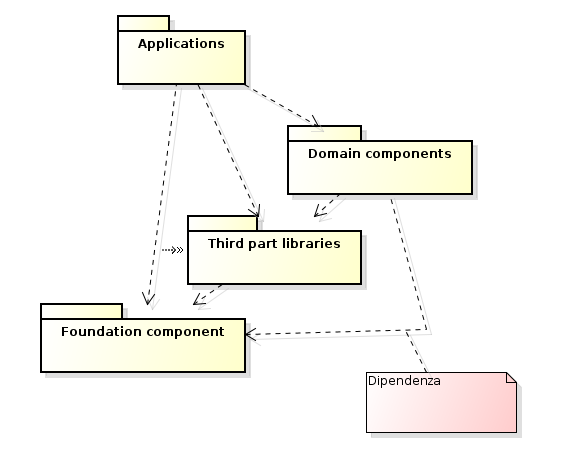
\includegraphics[width=0.75\columnwidth]{img3} % Example image

\end{center}

Caratteristiche:

\begin{itemize}

	\item Tutte le dipendenze dovrebbero seguire la stessa direzione, a meno di isolamento voluto da sottostrutture;
	\item Evitare le dipendenze circolari;
	\item Relazioni di dipendenza non soltanto transitive, se modifico \textit{aaa} non necessariamente modifico \textit{ccc};
	\item Più dipendenze entranti, più il \textit{package} dovrebbe essere stabile.

\end{itemize}

\textbf{Esempio}:\\
\textit{Il cliente sfoglia il catalogo ed aggiunge i prodotti desiderati al carrello della spesa. Quando il cliente termina l’acquisto e deve pagare, lo stesso fornisce le informazioni sulla consegna dei prodotti e sulla carta di credito. Il sistema verifica l’autorizzazione al pagamento con carta di credito e conferma l’acquisto immediatamente e mediante una successiva mail.
}

\begin{center}

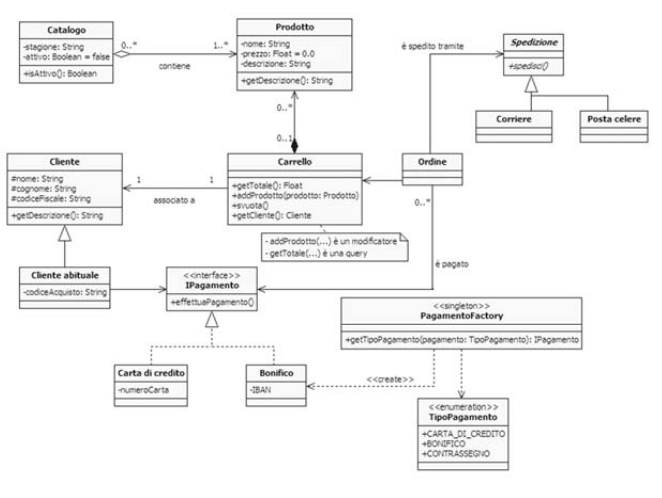
\includegraphics[width=0.75\columnwidth]{img4} % Example image

\end{center}

\begin{center}

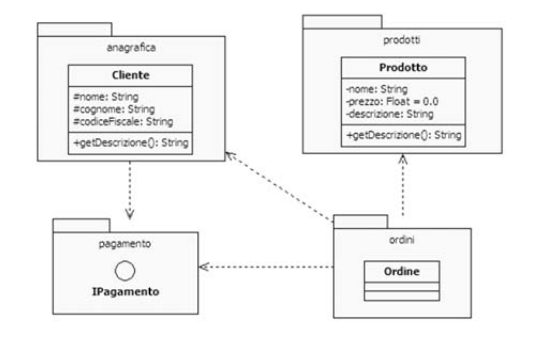
\includegraphics[width=0.75\columnwidth]{img5} % Example image

\end{center}


\end{document}